\section{Results} 
Decision trees emerge as the most accurate ML algorithm for classifying encrypted VoD traffic \cite{orsolic2018youtube} \cite{dimopoulos2016measuring} \cite{orsolic2017machine}. We used a Decision Tree model to predict video spatial resolution. The different spatial resolution labels that have been observed are: 1280x720, 1120x630, 960x540, 800x450, 640x360, 480x270, and 320x180. We used the Gini \cite{gini1936measure} index as a classification criterion. It measures the split quality - let the data at node m be represented by $Q_m$ with $N_m$ samples, let the target be a classification outcome with possible values $0, 1, …., K-1$, then for node m, let the term of \cref{eq:pm} be the proportion of class k observations in node m. If m is a terminal node, predicted probability for this region is set to $p_{mk}$. And the measure of impurity is represented by \cref{eq:hqm}. We used best split as the splitter strategy at each node.

\begin{equation}
    p_{mk} = \frac{1}{N_m}\sum_{y \in Q_m}I(y=k)
    \label{eq:pm}
\end{equation}

\begin{equation}
    H(Q_m) = \sum_k p_{mk}(1-p_{mk})
    \label{eq:hqm}
\end{equation}
We further calculated Permutation Feature Importance, to understand which features are more dominant for the QoE prediction. Permutation Feature Importance provides a score for each feature, whereas the highest the score, the more relevant the feature is for predicting the output label. The permutation feature importance is a model agnostic approach, calculated by noticing the increase or decrease in error when we permute the values of a feature. If permuting the values cause a huge change in the error, it means the feature is important for our model. The permutation feature importance is based on an algorithm that works as follows: (1) Calculate the mean squared error between the model results and the known labels with the original values; (2) Permute the values for the features and make predictions again; (3) Calculate the mean squared error with the shuffled values; (4) Compare the difference between them; (5) Sort the differences in descending order to get features with most to least importance.
The results are depicted in \Cref{fig:feat-import} and indicate that the bandwidth (Bits Per Second) represents the most dominant feature but Packet Length and Average Time Between Packets fall not far behind.
To gain better understanding of the features and their impact on the classification result, we performed a correlation check between the three most dominant features. As can be seen in \Cref{fig:feat-corr}, the correlation between the three dominant features is high, so we can conclude that the most applicable feature is the bandwidth. We used a Decision Tree model for classification of the video resolution. The rest of the QoE labels – fps, NIQE, Latency and Jitter are represented by integer values, which are more suitable for regression. We compared the results of a regression algorithm to those of Artificial Neural Network and found the later to be more accurate. The accuracy of our results is provided in \cref{tab:final_accuracy}. The network was created using the "Sequential" module of the Keras library. The used fully connected network is depicted in \Cref{fig:nn-arch}.
For the regression network we have used the ReLU activation function, batch size 20, and 50 Epochs. We used the 'Adam' optimizer.
The accuracy was calculated by applying the trained model to each row of testing dataset (30\% of the data samples) as the Absolute Percentage Error. We calculated the average of all the rows to obtain the Mean Absolute Percentage Error (MAPE). We further calculated Permutation Feature Importance, to understand which features are more dominant for the QoE prediction. Permutation Feature Importance provides a score for each feature, whereas the highest the score, the more relevant the feature is for predicting the output label. The permutation feature importance is a model agnostic approach, calculated by noticing the increase or decrease in error when we permute the values of a feature. If permuting the values cause a huge change in the error, it means the feature is important for our model. The permutation feature importance is based on an algorithm that works as follows: (1) Calculate the mean squared error between the model results and the known labels with the original values; (2) Permute the values for the features and make predictions again; (3) Calculate the mean squared error with the shuffled values; (4) Compare the difference between them; (5)	Sort the differences in descending order to get features with most to least importance.
The results are depicted in \Cref{fig:feat-import} and indicate that the bandwidth (Bits Per Second) represents the most dominant feature but Packet Length and Average Time Between Packets fall not far behind.

\begin{figure}
    \centering
    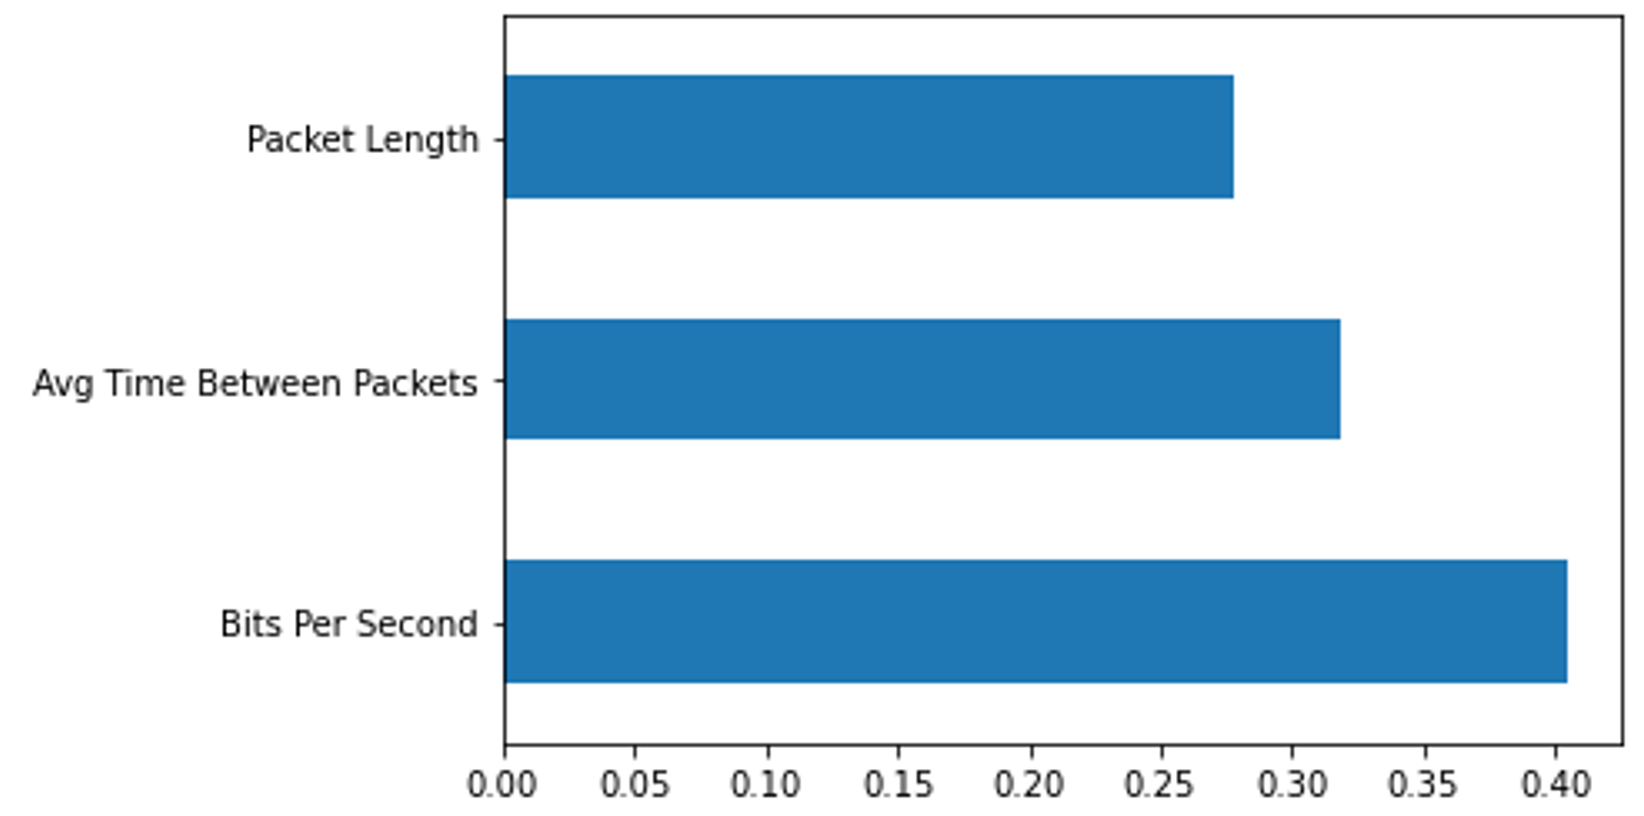
\includegraphics[scale=0.18]{feat_import.png}
    \caption{Feature importance calculation}
    \label{fig:feat-import}
\end{figure}

To gain better understanding of the features and their impact on the classification result, we performed a correlation check between the three most dominant features. As can be seen in \Cref{fig:feat-corr}, the correlation between the three dominant features is high, so we can conclude that the most applicable feature is the bandwidth. We used a Decision Tree model for classification of the video resolution. 

We trained a deep neural network with 16-64 layers and 128-256 units in each layer, as shown in \cref{fig:nn-arch}. We split the data into train and test dataset with a proportion of 90:10\%, while the train data was further split each train procedure with proportion of 80:20\% for the train data and validation respectively to monitor the performance in the course of the training. 
Parameter selection was done by a 5-fold cross validation where each time the train and test data was chosen anew in a non-overlapping manner (i.e., the tests of all the 5 folds were cohosen as non-overlapping sets).
The performance of the NN are summarized in \cref{tab:ablation}, for each of the predicted labels, viz. NIQE, Resolution and FPS.
% The rest of the QoE labels – fps, NIQE, Latency and Jitter are represented by integer values, which are more suitable for regression. We compared the results of a regression algorithm to those of Artificial Neural Network and found the later to be more accurate. 
% The accuracy of our results is provided in Table 1. The network was created using the "Sequential" module of the Keras library. The used fully connected network is depicted in \Cref{fig:nn-arch}.
% For the regression network we have used the ReLU activation function, batch size 20, and 50 Epochs. We used the 'Adam' optimizer.
% The accuracy was calculated by applying the trained model to each row of testing dataset (30\% of the data samples) as the Absolute Percentage Error. We calculated the average of all the rows to obtain the Mean Absolute Percentage Error (MAPE).

\begin{table}[]
    \centering
    \caption{QoE prediction accuracy results}
    \begin{tabular}{l|l|c}
        Predicted Label & Model & Accuracy \\
        \hline
        Resolution & DT & 90.489\% \\
        FPS & NN & 92.492\% \\
        NIQE & NN & 97.643\% \\

    \end{tabular}
    \label{tab:final_accuracy}
\end{table}

\begin{figure}
    \centering
    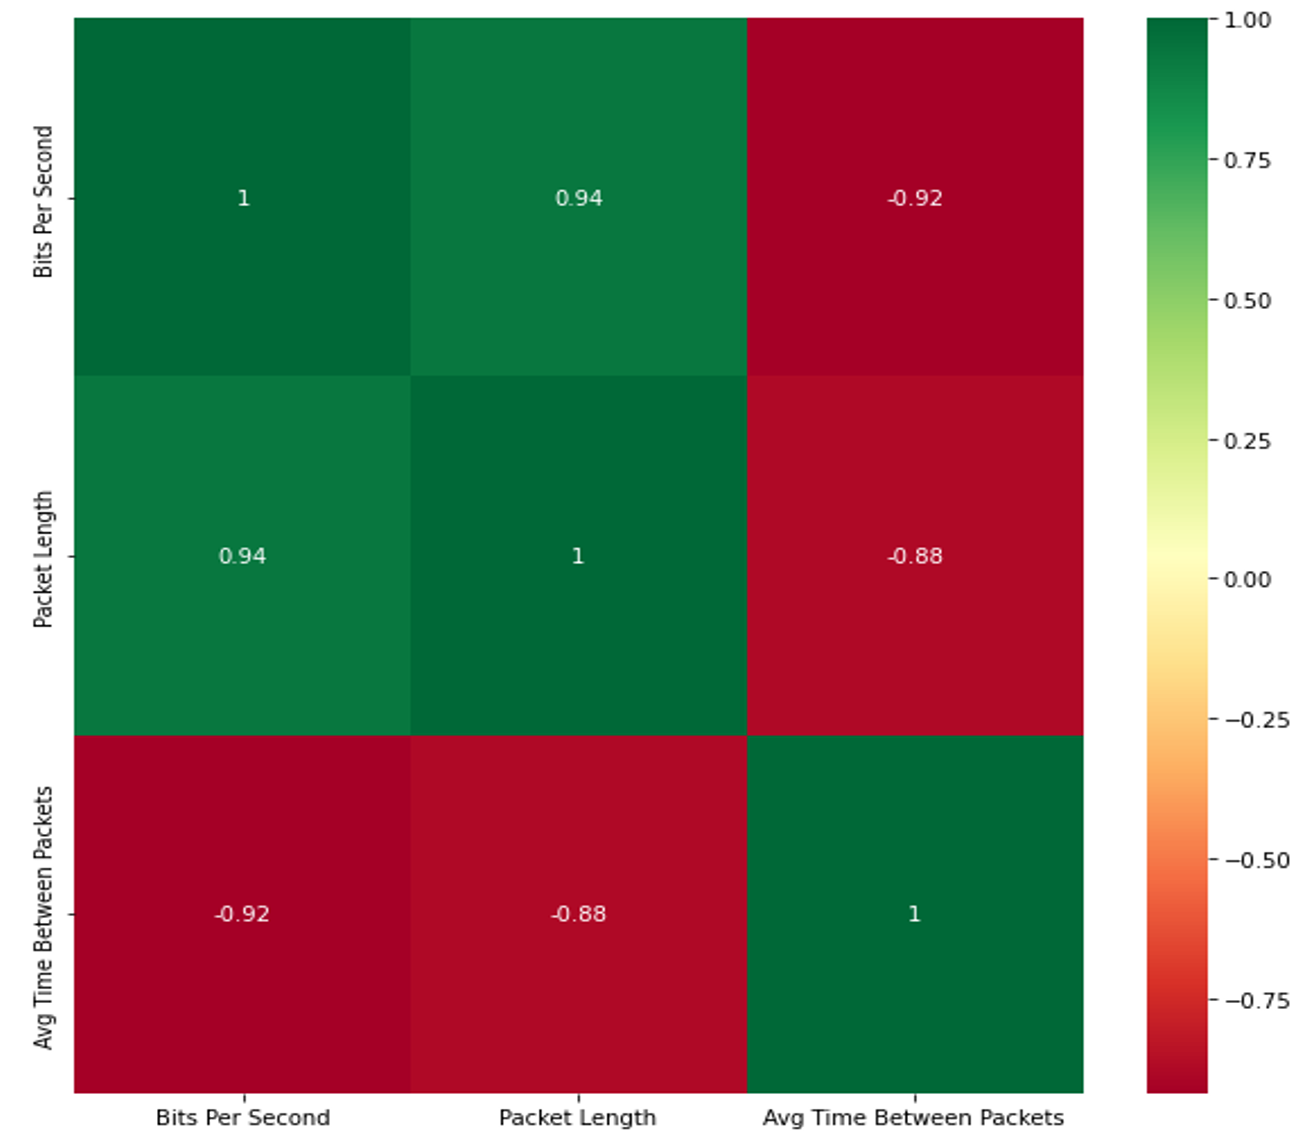
\includegraphics[scale=0.25]{conf_mat.png}
    \caption{Correlation between features}
    \label{fig:feat-corr}
\end{figure}

\begin{figure*}
    \centering
    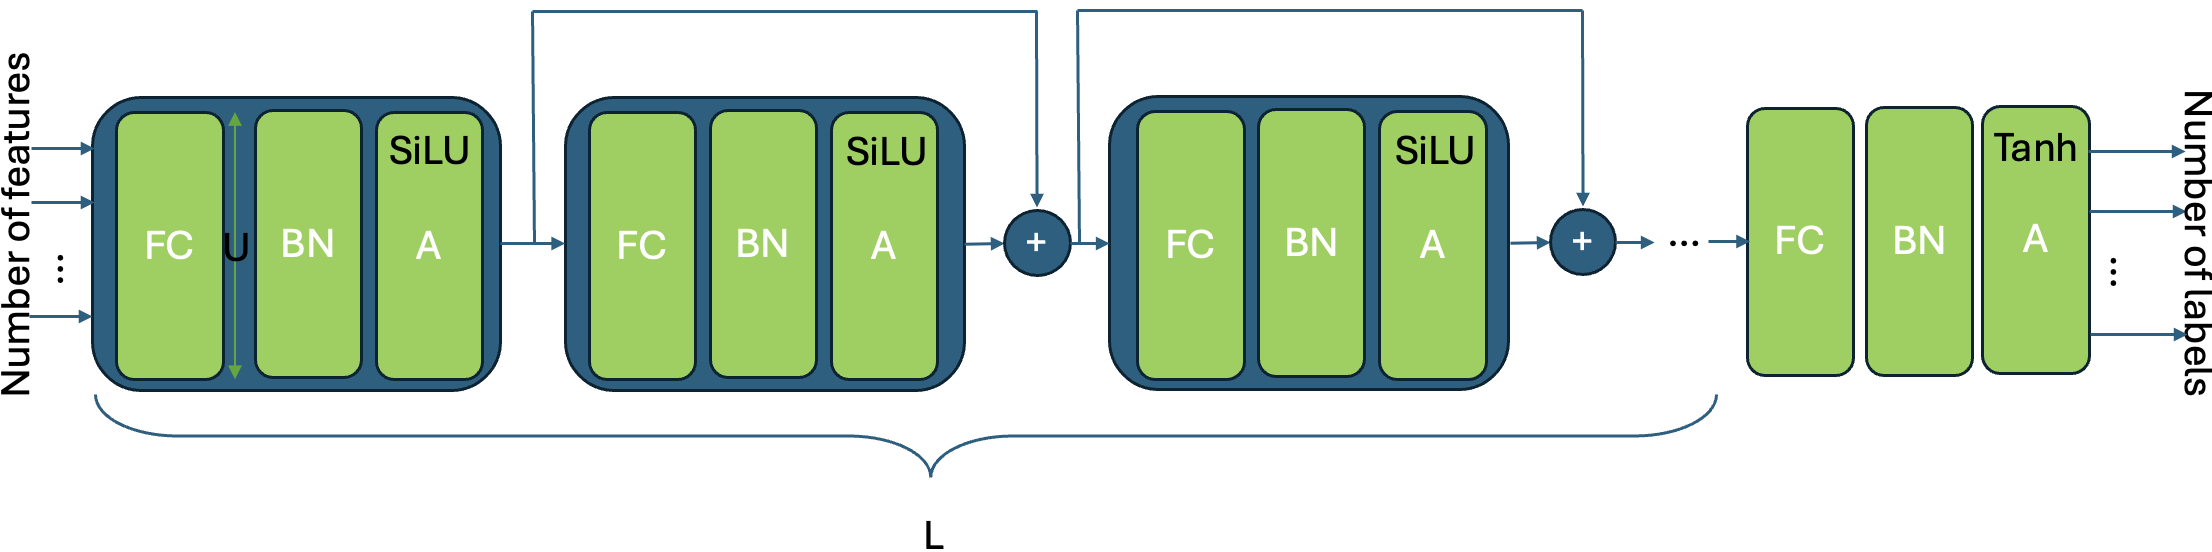
\includegraphics[scale=0.45]{figures/QNN Design.png}
    \caption{QoE prediction Neural Network architecture}
    \label{fig:nn-arch}
\end{figure*}